\newcommand{\makeSampleFig}{%
\begin{figure}[tb]
 \centering % avoid the use of \begin{center}...\end{center} and use \centering instead (more compact)
 \includegraphics[width=\columnwidth]{sample}
 \caption{A visualization of the 1990--2015 data from \autoref{tab:vis_papers}. The image is from \cite{Isenberg:2017:VMC} and is in the public domain.}
 \label{fig:sample}
\end{figure}}

\newcommand{\makeBasicPlottingFig}{%
\begin{figure}[!htbp]
 \centering
 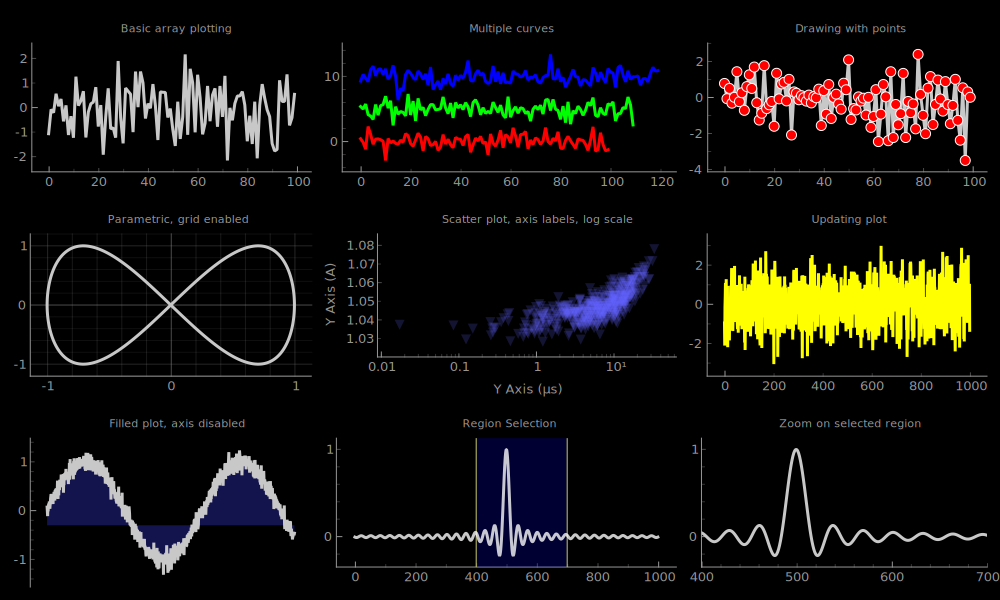
\includegraphics[width=\columnwidth]{basicPlotting}
 \caption{A caption.}
 \label{fig:basicPlotting}
\end{figure}}